\documentclass[,a4paper]{article}
\usepackage{geometry}
\geometry{a4paper,left=35mm,right=35mm, top=25mm, bottom=25mm}
\usepackage[T1]{fontenc}
\usepackage{lmodern}
\usepackage{amssymb,amsmath}
\usepackage{ifxetex,ifluatex}
\usepackage{fixltx2e} % provides \textsubscript
% use microtype if available
\IfFileExists{microtype.sty}{\usepackage{microtype}}{}
\ifnum 0\ifxetex 1\fi\ifluatex 1\fi=0 % if pdftex
  \usepackage[utf8]{inputenc}
\else % if luatex or xelatex
  \usepackage{fontspec}
  \ifxetex
    \usepackage{xltxtra,xunicode}
  \fi
  \defaultfontfeatures{Mapping=tex-text,Scale=MatchLowercase}
  \newcommand{\euro}{€}
\fi
% Redefine labelwidth for lists; otherwise, the enumerate package will cause
% markers to extend beyond the left margin.
\makeatletter\AtBeginDocument{%
  \renewcommand{\@listi}
    {\setlength{\labelwidth}{4em}}
}\makeatother
\usepackage{enumerate}
\usepackage{graphicx}
% We will generate all images so they have a width \maxwidth. This means
% that they will get their normal width if they fit onto the page, but
% are scaled down if they would overflow the margins.
\makeatletter
\def\maxwidth{\ifdim\Gin@nat@width>\linewidth\linewidth
\else\Gin@nat@width\fi}
\makeatother
\let\Oldincludegraphics\includegraphics
\renewcommand{\includegraphics}[1]{\Oldincludegraphics[width=\maxwidth]{#1}}
\ifxetex
  \usepackage[setpagesize=false, % page size defined by xetex
              unicode=false, % unicode breaks when used with xetex
              xetex]{hyperref}
\else
  \usepackage[unicode=true]{hyperref}
\fi
\hypersetup{breaklinks=true,
            bookmarks=true,
            pdfauthor={Marian Steinbach marian@sendung.de},
            pdftitle={Entwurf eines Standards für Datenmodell und Zugriffs-Protokoll für offene Ratsinformationssysteme},
            colorlinks=true,
            urlcolor=blue,
            linkcolor=magenta,
            pdfborder={0 0 0}}
\setlength{\parindent}{0pt}
\setlength{\parskip}{6pt plus 2pt minus 1pt}
\setlength{\emergencystretch}{3em}  % prevent overfull lines
\setcounter{secnumdepth}{0}

\title{Entwurf eines Standards für Datenmodell und Zugriffs-Protokoll für
       offene Ratsinformationssysteme}
\author{Marian Steinbach
                \href{mailto:marian@sendung.de}{\texttt{marian@sendung.de}}}
\date{}

\begin{document}
\maketitle

Lizenz: Creative Commons CC-BY-SA

\section{Einleitung}

\subsection{Ziel dieses Dokuments}

Ziel dieses Dokuments ist es, einen Diskurs über einen offenen Standard
zum Datenabruf aus Ratsinformationssystemen in Gang zu bringen.

Ratsinformationssysteme (RIS) werden von vielen Körperschaften wie
Kommunen, Landkreisen und Regierungsbezirken eingesetzt, um die
anfallende Gremienarbeit (Ratssitzungen, Ausschüsse, Vertretungen) zu
organisieren. Da ein großer Teil der schriftlichen Arbeit der
Lokalpolitik über derartige Systeme verwaltet wird, sind die RIS -- dort
wo vorhanden -- ein wichtiger Zugriffspunkt für alle, die sich für
politischen Geschehnisse interessieren.

Eine wichtige Maßnahme von Körperschaften, die im Zuge von Open-Data-
und Open-Government-Initiativen ihre Politik transparenter machen
wollen, wird auch sein, die Daten in den RIS im Sinne des
Open-Data-Begriffs zugänglich zu machen. Hierdurch können die Kommunen
selbst, aber auch dritte, Anwendungen entwickeln, die Inhalte auf
verschiedene Art und Weise auswerten, abrufbar und nutzbar machen, sei
es für die Allgemeinheit oder für bestimmte Nutzerkreise.

In Deutschland gibt es über 10.000 Kommunen, außerdem hunderte weitere
Körperschaften, die potenziell über RIS-ähnliche Systeme verfügen.
Sollten diese beginnen, ihre RIS zu öffnen, werden sie sämtlich vor der
Frage stehen, wie Daten zu modellieren und Schnittstellen (APIs) zu
spezifizieren sind.

Sowohl die Anbieter der Daten, als auch die Abnehmer (die
Anwendungsentwickler) werden von einer Standardisierung der
Schnittstellen und Datenmodelle profitieren. So wird die Kompatibilität
von Software und die breite Einsetzbarkeit ermöglicht.

Dieses Dokument soll die Erarbeitung eines solchen Standards ermöglichen
und als Diskussionsgrundlage dienen.

\subsection{Status}

Dieser Entwurf gibt aktuell einen ersten Vorschlag des Autors wieder. Es
ist vereinzelt Feedback eingeflossen (siehe ``Mitwirkende'').

\subsection{Überblick}

Der Entwurf umfasst im ersten Schritt die abstrakte Beschreibung eines
Datenmodells.

\subsubsection{Noch nicht abgedeckt:}

\begin{itemize}
\item
  Angaben von Personen zu Tätigkeiten (z.B. Auskunft nach § 17
  Korruptionsbekämpfungsgesetz). Diese werden von mehreren Systemen
  geführt und ausgegeben.
\item
  Änderungsdatum (bei allen Objekttypen relevant)
\item
  Unterscheidung von Rollen bzw. Zuständigkeiten zwischen Drucksachen
  und Tagesordnungspunkten (z.B. federführende Beratung, konsultierende
  Beratung etc.)
\end{itemize}

\subsection{Nächste Schritte}

\begin{enumerate}[1.]
\item
  Bis Ende Mai 2012: Einsammeln von Feedback zum Entwurf des
  Datenmodells
\item
  Anpassen des Entwurfs anhand von Feedback
\item
  Erarbeitung eines Entwurfs für eine HTTP-basierte Schnittstelle zum
  lesenden Zugriff auf Daten. Darin soll beschrieben werden, wie über
  HTTP die zuvor beschriebenen Daten abgerufen werden sollen.
\end{enumerate}

\subsection{Feedback}

Feedback wird dringend benötigt und ist daher herzlichst willkommen.
Feedback kann auf den folgenden Wegen eingereicht werden:

\begin{itemize}
\item
  Als Pull Requests über Github, direkt am Quelltext
\item
  Über Issues auf Github
\item
  Per E-Mail
\end{itemize}

\subsubsection{Pull Requests über Github}

Dieses Dokument wird in folgendem Github-Repository gepflegt:

\href{https://github.com/marians/open-ris-specs}{https://github.com/marians/open-ris-specs}

Der bevorzugte Feedback-Kanal für erfahrene Git- bzw. Github-Nutzer ist
entsprechend die Mitwirkung direkt am Quelltext in Form von
Pull-Requests. So können \textbf{Ergänzungen und Korrekturen} direkt in
den Quelltext eingespielt werden.

Ausführliche Anleitungen zur Arbeit mit Git/Github finden sich auf der
Plattform selbst sowie an vielen Orten im Netz. Der allgemeine Ablauf
ist wie folgt:

\begin{enumerate}[1.]
\item
  Erzeugen Sie sich, sofern noch nicht geschehen, ein Benutzerkonto auf
  Github.
\item
  Duplizieren (\emph{forken}) Sie das oben genannte Repository
\item
  Nehmen Sie die gewünschten Änderungen an Ihrem Repository vor.
  Committen Sie diese Änderungen möglichst kleinteilig.
\item
  Senden Sie die gewünschten Commits als Pull Requests.
\end{enumerate}

Als Autor werde ich entscheiden, welche Pull Requests ich übernehme. Sie
werden als Mitwirkender in diesem Dokument genannt. Wenn Sie mit einen
Klarnamen unggf. Unternehmenszugehörigkeit genannt werden wollen, teilen
Sie mir dies bitte per Mail an marian@sendung.de mit.

\subsubsection{Issues auf Github}

Wer nicht über Github am Quelltext mitwirken möchte, aber einen
Github-Account sein eigen nennt (oder zu diesem Zweck anlegen möchte)
und \textbf{öffentlich kommentieren} möchte, der sollte das öffentliche
Issue-Tracking-System unter

\href{https://github.com/marians/open-ris-specs/issues}{https://github.com/marians/open-ris-specs/issues}

verwenden. Vorteil daran ist, dass auch andere die Einträge lesen und
wiederum durch Kommentare ergänzen können. Zudem lässt sich der
Bearbeitungsstatus eines Issue-Eintrags (offen, geschlossen) nachhalten.

Bitte achten Sie auf diesem Weg darauf, Ihre Kommentare in möglichst
kleine thematische Einheiten herunter zu brechen.

\subsubsection{Feedback per E-Mail}

Sollten Sie keinen der oben beschriebenen Wege beschreiten wollen,
können Sie Anmerkungen zum Dokument per E-Mail an marian@sendung.de
einsenden. Bitte verwenden Sie dabei den Begriff ``open-ris-specs'' im
Betreff.

Sollten Sie auf diesem Wege Anmerkungen direkt am/im Dokumententext
übersenden wollen, nutzen Sie bitte falls möglich die Word- oder
OpenOffice-Version dieses Dokuments und ändern Sie das Dokument so, dass
Änderungen aufgezeichnet werden (OpenOffice: Bearbeiten \textgreater{}
Änderungen \textgreater{} Aufzeichnen; Word: Ribbon ``Überprüfen''
\textgreater{} Nachverfolgung \textgreater{} Änderungen nachverfolgen).

\subsection{Mitwirkende}

Felix Ebert, Jan Erhardt

\section{Datenmodell}

Das Datenmodell soll die Bausteine für die später zu entwerfende
Schnittstelle definieren. Im folgenden werden sozusagen die Objekttypen
bzw. die Klassen beschrieben, auf die über eine spätere API zugegriffen
werden kann.

Einige Objekte werden eine eindeutige Identifizierung (ID) benötigen,
wobei „eindeutig`` auch eine Frage des Kontextes ist. In den wenigsten
Fällen wird es notwendig sein, eine Objekt-Kennung weltweit eindeutig zu
machen. Darüber hinaus wird zu entscheiden sein, ob IDs unveränderlich
oder veränderlich sein sollen.

Die Hinweise auf die Praxis in bestehenden Ratsinformationssystemen
beziehen sich auf nach außen, bei Nutzung der jeweiligen Weboberflächen,
feststellbare Eigenschaften. Dabei wird vereinzelt und beispielhaft auf
die folgenden Systeme Bezug genommen:

\begin{itemize}
\item
  Stadt Köln {[}2{]} - Plattform: Somacos SessionNet {[}3{]}
\item
  Bezirksverwaltung Berlin Mitte {[}4{]} - Plattform: ALLRIS {[}5{]}
\item
  Stadt Rösrath {[}6{]} - Plattform der Firma PROVOX {[}7{]}
\item
  Stadt Euskirchen {[}8{]} - Plattform: SD.NET RIM 4 {[}9{]}
\item
  Stadt Bonn - BoRis {[}10{]}
\end{itemize}

\subsubsection{Zu den Eigenschaften}

Eigenschaften der einzelnen Objekttypen sind, wenn nicht anders
angegeben, verpflichtend. Optionale Eigenschaften sind entsprechend
gekennzeichnet.

Durch die aktuelle Detailtiefe der Beschreibungen soll vor allem die
Frage ``Was soll/kann gespeichert bzw. ausgedrückt werden?'' geklärt
werden.

Detailliertere Anforderungen an die Eigenschaften (``Wie genau soll eine
Information gespeichert werden?'') werden zu einem späteren Zeitpunkt
erörtert.

Eigenschaften werden aktuell deutschsprachig benannt. Es wird
beabsichtigt, die Benennungen zu einem späteren Zeitpunkt im
Entwurfsprozess gegen Eenglischsprachige Begriffe auszutauschen.

\subsubsection{Zu den Beziehungen}

Bei Beschreibung der Beziehungen zwischen Objekten wird zu diesem
Zeitpunkt nicht berücksichtigt, ob eine Beziehung zwischen zwei Objekten
A und B am Objekt A oder am Objekt B definiert wird. So spielt es
bislang keine Rolle, ob einem Gremium mehrere Personen zugeordnet werden
oder einer Person mehrere Gremien zugewiesen werden. Das Augenmerkt
liegt hier nur auf der Tatsache, welche Beziehung existieren können und
was diese Beziehungen aussagen sollen.

\subsection{Gebietskörperschaft}

Die Gebietskörperschaft erlaubt es, Körperschaften wie einen bestimmten
Landkreis, eine bestimmte Gemeinde oder einen bestimmten Stadtbezirk in
Form eines Datenobjekts abzubilden.

Viele RIS werden nur genau eine Instanz dieses Typs „beherbergen``.
Einige Systeme werden jedoch für mehrere Mandanten betrieben, wobei die
Mandanten verschiedene Gebietskörperschaften repräsentieren
(z.B.''Verbandsgemeinde Ulmen" und ``Stadt Ulmen''.)

\begin{figure}[htbp]
\centering
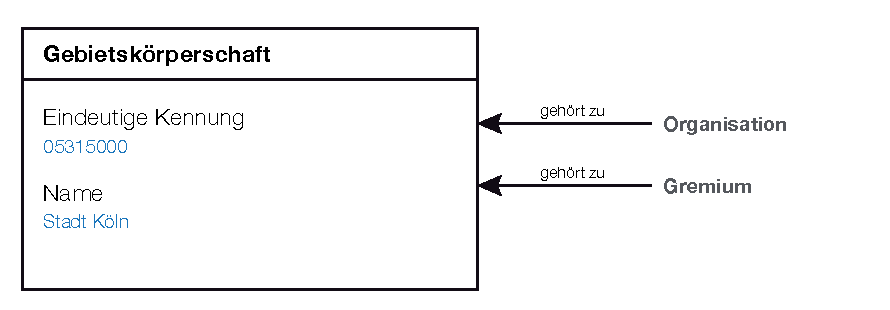
\includegraphics{images/datenmodell_gebietskoerperschaft.pdf}
\caption{Objekttyp Gebietskörperschaft}
\end{figure}

\subsubsection{Eindeutige Identifizierung}

Zur Identifizierung des Objekts kann der Amtliche Gemeindeschlüssel
(AGS{[}1{]}) verwendet werden, der alle deutschen Gemeinden, Landkreise,
kreisfreien Städte etc. eindeutig erfasst.

Vorteil der Verwendung des AGS:

\begin{itemize}
\item
  Kompakte, einfache und einheitliche Schreibweise für jede
  Körperschaft.
\item
  Der AGS wird von Behörden genutzt, ist anerkannt und auch in anderen
  Medien, z.B. der Wikipedia, verbreitet.
\end{itemize}

Nachteil des AGS:

\begin{itemize}
\item
  Führende Nullen machen den Schlüssel fehleranfällig. Bestimmte Systeme
  wie z.B. Excel könnten den Inhalt als Zahlenwert erkennen und die
  führenden Nullen automatisch verwerfen.
\item
  Für Gebietsgliederungen unterhalb der selbstständigen Gemeinde,
  beispielsweise einen einzelnen Stadtbezirk, gibt es keinen eigenen
  Gemeindeschlüssel. Dies müssten durch eine nicht-amtliche Erweiterung
  des Systems ausgeglichen werden.
\end{itemize}

\subsubsection{Eigenschaften}

\begin{description}
\item[Name]
Der Name der Gebietskörperschaft, z.B. ``Köln'' oder ``Stadt Köln''.
\end{description}

\subsubsection{Beziehungen}

\begin{itemize}
\item
  Objekte vom Typ ``Organisation'' sind zwingend genau einer
  Gebietskörperschaft zugeordnet. So wird beispielseise eine SPD in Köln
  von einer SPD in Leverkusen unterschieden.
\item
  Objekte vom Typ ``Gremium'' sind zwingend genau einer
  Gebietskörperschaft zugeordnet. Damit wird der ``Rat'' einer
  bestimmten Kommune von den gleichnamigen Gremien anderer Kommunen
  abgegrenzt.
\end{itemize}

\subsection{Gremium}

Das Gremium ist ein Personenkreis, üblicherweise von gewählten und/oder
ernannten Mitgliedern. Beispiele hierfür sind der Stadtrat, Kreisrat,
Gemeinderat, Ausschüsse und Bezirksvertretungen. Gremien halten
Sitzungen ab, zu denen die Gremien-Mitglieder eingeladen werden.

\begin{figure}[htbp]
\centering
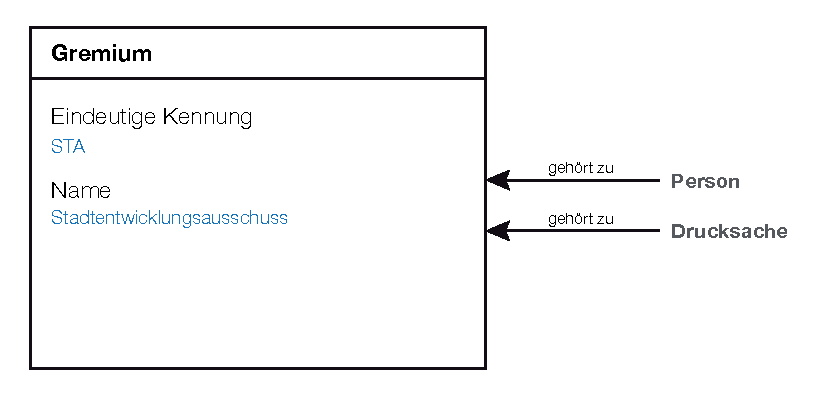
\includegraphics{images/datenmodell_gremium.pdf}
\caption{Objekttyp Gremium}
\end{figure}

\subsubsection{Eigenschaften}

\begin{description}
\item[Kennung]
Zur eindeutigen Identifizierung des Gremiums im Kontext einer bestimmten
Gebietskörperschaft. Die Stadt Köln verwendet beispielswiese das Kürzel
``STA'' für den Stadtentwicklungsausschuss oder ``BA'' für den Ausschuss
für Anregungen und Beschwerden. Andere Kommunen verwenden z.B. rein
numerische Kennungen.
\item[Name]
Der Name des Gremiums. Beispiele: ``Rat'', ``Hauptausschuss'',
``Bezirksvertretung 1 (Innenstadt)''
\end{description}

\paragraph{Anmerkungen}

Beim Rösrather RIS {[}6{]} wird für jedes Gremium ein Kurz- und ein
Langname angegeben. Beispielsweise wird beim ``Stadtentwicklungs-,
Planungs- und Verkehrsausschuss'' die kurze Form ``Stadtentwicklung''
hinterlegt. Bei 5 von 12 Gremien sind jedoch Kurz- und Langnamen
identisch.

Sofern nicht Beispiele aus weiteren Systemen vorliegen, wird dieser
Einzelfall nicht im Entwurf abgebildet.

\subsubsection{Beziehungen}

\begin{itemize}
\item
  Objekte vom Typ ``Person'' referenzieren auf Gremien, um die
  Mitgliedschaft/Zugehörigkeit einer Person im/zum Gremium zu
  kennzeichnen.
\item
  Objekte vom Typ ``Drucksache'' können einem Gremium zugeordnet sein.
  Beispielsweise wird eine Anfrage oder ein Antrag dem Rat oder einer
  bestimmten Bezirksvertretung zugeordnet.
\end{itemize}

\subsection{Person}

Jede natürliche Person, die Mitglied eines Gremiums ist, ist als Person
im Datenmodell eindeutig identifizierbar.

\begin{figure}[htbp]
\centering
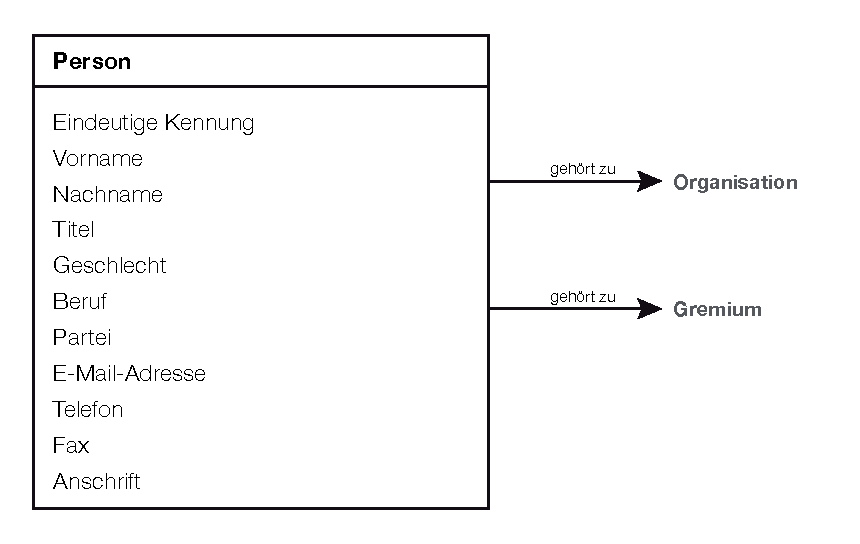
\includegraphics{images/datenmodell_person.pdf}
\caption{Objekttyp Person}
\end{figure}

\subsubsection{Eigenschaften}

\begin{description}
\item[Kennung]
Zur eindeutigen Identifizierung sollte jede Person eine Kennung
besitzen, die keinen Änderungen unterworfen ist und aus diesem Grund
nicht mit dem Namen in Verbindung stehen sollte. Viele RIS nutzen rein
numerische Kennungen.
\item[Vorname]
Der Vorname der Person.
\item[Nachname]
Der Nachname der Person.
\item[Titel]
\emph{Optional}. Akademische Titel wie ``Dr.'' und ``Prof.~Dr.''
\item[Geschlecht]
\emph{Optional}. Männlich/Weblich
\item[Beruf]
\emph{Optional}. Z.B. ``Rechtsanwalt''
\item[Partei]
\emph{Optional}. Z.B. ``Bündnis 90/Grüne''
\item[E-Mail-Adresse]
\emph{Optional}.
\item[Telefon]
\emph{Optional}.
\item[Fax]
\emph{Optional}.
\item[Anschrift]
\emph{Optional}. Straße und Hausnummer, Postleitzahl und Ort
\end{description}

\paragraph{Anmerkungen}

\begin{itemize}
\item
  Das System von Euskirchen scheint Vor- und Nachname (evtl. einschl.
  Titel) in einem gemeinsamen Feld ``Name'' zu führen. Ob das System
  hier technisch differenziert, ist unklar. Falls einzelne Systeme den
  angezeigten Namen nur als ganzes speichern, sollte dies für den
  Standard übernommen werden, da es für die meisten Anwendungen
  ausreichen sollte.
\item
  Das System PROVOX unterscheidet zwischen privaten und geschäftlichen
  Anschriften.
\end{itemize}

\subsubsection{Beziehungen}

\begin{itemize}
\item
  Objekte vom Typ ``Person'' können einer Organisation, z.B. einer
  Fraktion, zugeornet werden. Diese Beziehung ist datiert.
\item
  Objekte vom Typ ``Person'' können einem oder mehreren Gremien
  zugewiesen werden, um die Mitgliedschaft in diesem Gremium
  darzustellen. Diese Beziehungen sind ebenfalls datiert.
\end{itemize}

\subsection{Organisation}

Organisationen sind üblicherweise Parteien bzw. Fraktionen, denen die
Personen angehören können.

\begin{figure}[htbp]
\centering
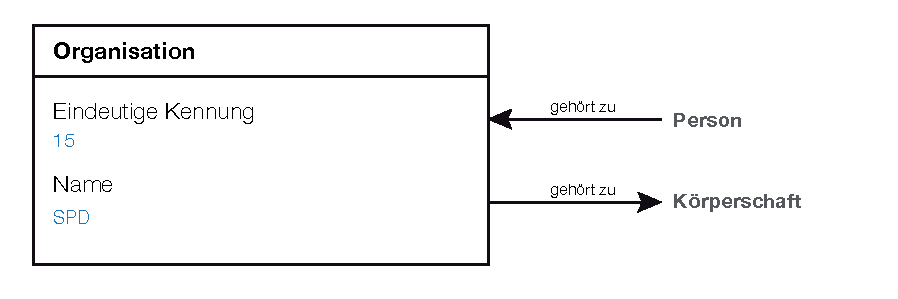
\includegraphics{images/datenmodell_organisation.pdf}
\caption{Objekttyp Organisation}
\end{figure}

\subsubsection{Eigenschaften}

\begin{description}
\item[Kennung]
Zur eindeutigen Kennzeichnung einer Organisation innerhalb einer
Gebietskörperschaft
\item[Name]
Der gebräuchliche Name der Organisation, z.B. ``SPD'' oder ``DIE
LINKE''.
\end{description}

\paragraph{Anmerkungen}

\begin{itemize}
\item
  Unklar ist bislang, ob Organisationen in der Praxis eher Fraktionen
  (``SPD-Fraktion im Kölner Rat'', ``SPD-Fraktion in Köln-Innenstadt'')
  abbilden oder ob eher Ortsverbände von Parteien (``SPD Köln'') gemeint
  sein werden. Einblicke, wie gängige Systeme dies handhaben, sollten
  evtl. gesammelt und berücksichtigt werden.
\end{itemize}

\subsubsection{Beziehungen}

\begin{itemize}
\item
  Jede Organisationen gehört zu einer Gebietskörperschaft.
\item
  Personen können Organisationen angehören (\emph{datiert}).
\end{itemize}

\subsection{Sitzung}

Eine Sitzung ist die Versammlung der Mitglieder eines Gremiums zu einem
bestimmten Zeitpunkt. Sitzungen können eine laufende Nummer haben.

Die geladenen Teilnehmer der Sitzung sind jeweils als „Person`` in
entsprechender Form referenziert. Verschiedene Drucksachen (Einladung,
Ergebnis- und Wortprotokoll) werden ebenfalls referenziert.

\begin{figure}[htbp]
\centering
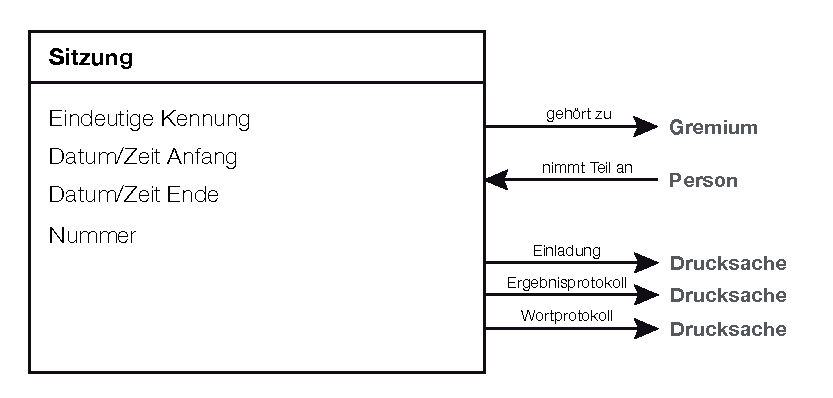
\includegraphics{images/datenmodell_sitzung.pdf}
\caption{Objekttyp Sitzung}
\end{figure}

\subsubsection{Eigenschaften}

\begin{description}
\item[Eindeutige Kennung]
Zur eindeutigen Identifizierung der Sitzung innerhalb einer
Gebietskörperschaft. In der Praxis wird eine solche Kennzeichnung
entweder durch eine laufende Nummer gebildet, oder durch Kombination
mehrerer Merkmale wie dem Kürzel des Gremiums, der laufenden Nummer der
Sitzung in einem Jahr und der Jahreszahl (z.B. ``BV1/0034/2012'').
\item[Nummer]
\emph{Optional}. Laufende Nummer der Sitzung, üblicherweise innerhalb
der Wahlperiode mit 1 beginnend. In der Praxis wird dadurch z.B. die
``2. Sitzung des Rats'' gekennzeichnet.
\item[Anfang]
Datum und ggf. Uhrzeit des Anfangszeitpunkts der Sitzung
\item[Ende]
\emph{Optional}. Datum und Uhrzeit vom Ende der Sitzung
\end{description}

\subsubsection{Beziehungen}

\begin{itemize}
\item
  Sitzungen sind grundsätzlich genau einem Gremium zugeordnet.
\item
  Personen sind Sitzungen zugeordnet, um die Teilnahme an der Sitzung
  auszudrücken.
\item
  Dokumente können vom Typ ``Sitzung'' \emph{optional} zu mehreren
  Zwecken referenziert werden:

  \begin{itemize}
  \item
    Zum Verweis auf die Einladung zur Sitzung
  \item
    Zum Verweis auf das Ergebnisprotokoll zur Sitzung
  \item
    Zum Verweis auf das Wortprotokoll zur Sitzung
  \end{itemize}
\item
  Weiterhin können Sitzungen beliebige weitere Dokumente, die keine
  eigenständigen Drucksachen sind, referenzieren.
\end{itemize}

\subsection{Tagesordnungspunkt}

Der Tagesordnungspunkt wird für eine bestimmte Sitzung angelegt, erhält
eine (innerhalb dieser Sitzung eindeutige) Nummer und einen Titel
(Betreff). Nach der Sitzung wird dem Tagesordnungspunkt außerdem ein
Ergebnis angehängt. Falls abweichend von der ursprünglichen
Beschlussvorlage (z.B. durch Berücksichtigung eines Änderungsantrags)
kann ein bestimmter Beschlusstext zu Protokoll gegeben werden. Sofern
das Abstimmungsergebnis nicht einstimmig ist, kann es durch mehrere
referenzierende Stimmabgaben festgehalten werden.

In der Praxis werden die meisten Sitzungen mehrere Tagesordnungspunkte
haben.

\begin{figure}[htbp]
\centering
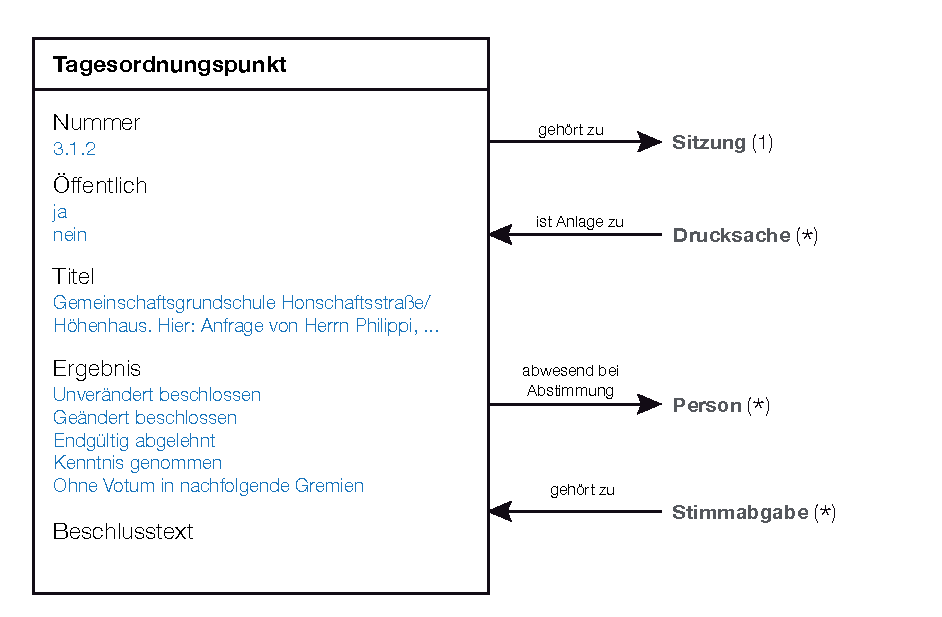
\includegraphics{images/datenmodell_tagesordnungspunkt.pdf}
\caption{Objekttyp Tagesordnungspunkt}
\end{figure}

\subsubsection{Eigenschaften}

\begin{description}
\item[Nummer]
Beispiel: ``1.2.3''. Diese Nummer gibt an, in welcher Reihenfolge die
Tagesordnungspunkte einer Sitzung behandelt werden. Im Kontext einer
Sitzung ist diese Nummer eindeutig.
\item[Öffentlich]
ja/nein. Kennzeichnet, ob der Tagesordnungspunkt in öffentlicher Sitzung
behandelt wird.
\item[Titel]
Das Thema des Tagesordnungspunktes
\item[Ergebnis]
Eines aus einer Liste definierter Ergebnisse. Möglich sind:
``Unverändert beschlossen'', ``Geändert beschlossen'', ``Endgültig
abgelehnt'', ``Zur Kenntnis genommen'', ``Ohne Votum in nachfolgende
Gremien überwiesen''
\item[Beschlusstext]
\emph{Optional}. Falls in diesem Tagesordnungspunkt ein Beschluss
gefasst wurde, kann der Text hier hinterlegt werden. Das ist besonders
dann in de Praxis relevant, wenn der gefasste Beschluss (z.B. durch
Änderungsantrag) von der Beschlussvorlage abweicht.
\end{description}

\paragraph{Anmerkungen}

\begin{itemize}
\item
  Einige Systeme vergeben zu Tagesordnungspunkten intern
  unveränderliche, numerische IDs. Es ist unklar, ob es zusätzlichen
  Nutzen bringt, derartige IDs, neben den Nummern, in den Standard zu
  übernehmen. Dies würde vermutlich nur Sinn ergeben, wenn es als
  Pflichtfeld gelten kann.
\end{itemize}

\subsubsection{Beziehungen}

\begin{itemize}
\item
  Jeder Tagesordnungspunkt gehört zu einer Sitzung.
\item
  Es können mehrere Objekte vom Typ ``Stimmabgabe'' referenziert werden,
  um das Abstimmungsverhalten von Fraktionen oder Einzelpersonen zu
  dokumentieren.
\item
  Es können Personen referenziert werden, die während der Abstimmung zu
  diesem Tagesordnungspunkt \emph{nicht} anwesend waren.
\end{itemize}

\subsection{Stimmabgabe}

Wie eine Person bzw. eine Fraktion zu einem Tagesordnungspunkt
abgestimmt hat, wird durch eine Stimmabgabe festgehalten. Ganze
Abstimmungsergebnisse bestehen überlicherweise aus mehreren
Stimmabgaben. Jede Stimmabgabe gibt entweder die (einzelne) Stimme einer
Peson wieder, in diesem Fall ist die Anzahl der Stimmen zwingend 1. Oder
eine Stimmabgabe gibt das Abstimmungsverhalten einer ganzen Gruppe von
Personen wieder. Dann ist die Anzahl der Stimmen anzugeben und statt
einer Person eine Organisation (in der Regel die Fraktion) zu
referenzieren.

\begin{figure}[htbp]
\centering
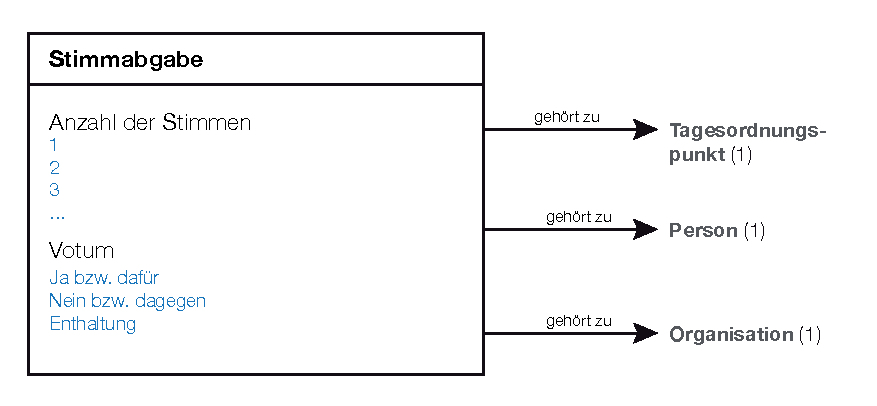
\includegraphics{images/datenmodell_stimmabgabe.pdf}
\caption{Objekttyp Stimmabgabe}
\end{figure}

\subsubsection{Eigenschaften}

\begin{description}
\item[Anzahl der Stimmen]
Gehört die Stimmabgabe zu einer Person, ist der Wert immer 1. Gehört sie
jedoch zu einer Organisation (=Fraktion), kann der Wert hier größer als
1 sein.
\item[Votum]
Einer der drei Werte ``ja'' (gleichbedeutend mit ``dafür''), ``nein''
(``dagegen'') oder ``Enthaltung''.
\end{description}

\subsubsection{Beziehungen}

\begin{itemize}
\item
  Jede Stimmabgabe gehört zu genau einem Tagesordnungspunkt.
\item
  Es wird entweder genau eine Person oder genau eine Organisation
  (Fraktion) referenziert, die die Stimme(n) abgegeben hat.
\end{itemize}

\subsection{Drucksache}

Eine Drucksache bildet Mitteilungen, Antworten auf Anfragen,
Beschlussvorlagen, Anfragen und Anträge ab. Jede Drucksache erhält eine
eindeutige Kennung.

Die Drucksache hat im Informationsmodell eine hervorgehobene Bedeutung.
Im Fall eines Antrags kann mit einer einzigen Drucksache ein über Monate
oder Jahre dauernder politischer Entscheidungsprozess verbunden sein. In
dem Zusammenhang entstehen üblicherweise weitere Drucksachen.

Drucksachen spielen in der schriftlichen wie mündlichen Kommunikation
eine besondere Rolle, da in vielen Texten auf bestimmte Drucksachen
Bezug genommen wird. Hierbei kommen in Ratsinformationssystemen
unveränderliche Kennungen der Drucksachen zum Einsatz.

\begin{figure}[htbp]
\centering
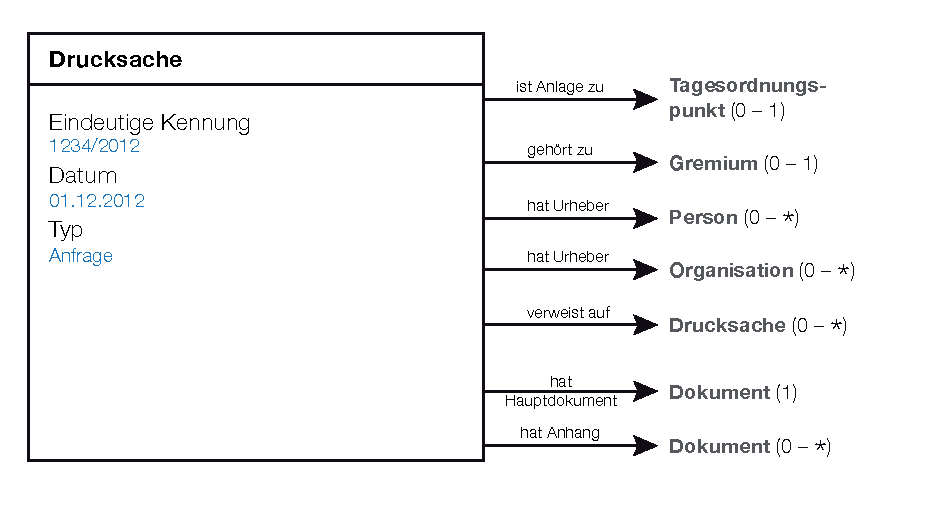
\includegraphics{images/datenmodell_drucksache.pdf}
\caption{Objekttyp Drucksache}
\end{figure}

Jede Drucksache ist über die Eigenschaft ``Typ'' als eine der folgenden
Arten von Drucksachen gekennzeichnet:

\begin{itemize}
\item
  \textbf{Beschlussvorlage}: Entscheidungsvorschlag der Verwaltung
\item
  \textbf{Antrag}: Entscheidungsvorschlag einer Fraktionen bzw. mehrerer
  Fraktionen oder einer/mehrerer Einzelperson/en
\item
  \textbf{Anfrage}: Frage(n) einer oder mehrerer Fraktion oder
  Einzelpersonen an die Verwaltung
\item
  \textbf{Mitteilung/Stellungnahme der Verwaltung}: Eine Information der
  Verwaltung an einzelne oder mehrere Gremien. Darunter fallen nicht
  Beantwortungen von Anfragen.
\item
  \textbf{Beantwortung einer Anfrage}: Antwort der Verwaltung auf
  (mündliche oder schriftliche) Anfragen
\end{itemize}

\subsubsection{Eigenschaften}

\begin{description}
\item[Kennung]
Die Kennung einer Drucksache muss für die jeweilige Gebietskörperschaft
eindeutig sein. Sie kann sowohl Ziffern als auch Buchstaben enthalten.
Einige Systeme (z.B. Köln) verwenden besondere Trennzeichen wie ``/'',
um eine Jahreszahl von einer laufenden Nummer abzutrennen. Weiterhin
werden mancherorts führende Nullen verwendet.
\item[Datum]
Datum der Veröffentlichung
\item[Typ]
Art der Drucksache (Erläuterung siehe oben)
\end{description}

\subsubsection{Beziehungen}

\begin{itemize}
\item
  Es muss genau ein \textbf{Hauptdokument} (Objekttyp ``Dokument'')
  referenziert werden.
\item
  Es können beliebig viele weitere Dokumente referenziert werden, die
  als nachgeordnete \textbf{Anlagen} zur Drucksache verstanden werden.
\item
  Es kann ein \textbf{Gremium} genannt werden, dem die Drucksache
  zuzuordnen ist. Hier ist zu klären, inwiefern dies für einzelne Typen
  von Drucksachen verpflichten sein sollte. So sollte beispielsweise
  eine Anfrage grundsätzlich aus einem Gremium (z.B. Gemeinderat)
  stammen.
\item
  Drucksachen können \textbf{Urhebern} zugewiesen werden. Im Fall von
  Mitteilungen der Verwaltung ist dies oft der Oberbürgermeister. Bei
  Anträgen oder Anfragen können Organisationen oder Einzelpersonen
  referenziert werden. Es können stets mehrere Ihrheber verknüpft
  werden.
\item
  Es können beliebig viele \textbf{Orte} (siehe Objekttyp ``Ort'')
  referenziert werden, die im Inhalt der Drucksache behandelt werden.
  Beispiel: Beschlussvorlage zur Freigabe von Mitteln für die Sanierung
  eines Sportplatzes, wobei der Ort die Lage des Sportplatzes genau
  beschreibt.
\item
  Beim Drucksachen-Typ ``Beantwortung einer Anfrage'' ist die Drucksache
  zu referenzieren, die die ursprüngliche \textbf{Anfrage} beinhaltet.
\item
  Drucksachen können zu beliebig vielen Tagesordnungspunkten in
  Beziehung stehen, um die \textbf{Beratungsfolge} einer Drucksache
  abzubilden. Hierbei kann die Beziehung jeweils mit einer
  Rollenbezeichnung versehen sein, die noch näher zu bestimmen ist
  (TODO).
\end{itemize}

\subsection{Dokument}

Ein Dokument hält die Daten und Metadaten einer Datei vor,
beispielsweise einer PDF-Datei, eines RTF- oder Word-Dokuments. Wird von
einem Word-Dokument eine PDF-Ableitung hinterlegt, ist diese Ableitung
ebenfalls ein Dokument, das jedoch nicht als Master gekennzeichnet wird,
sondern auf den entsprechenden Master verweist.

Im Unterschied zur Drucksache benötigt das Dokument keine
nutzerfreundliche Kennung.

\begin{figure}[htbp]
\centering
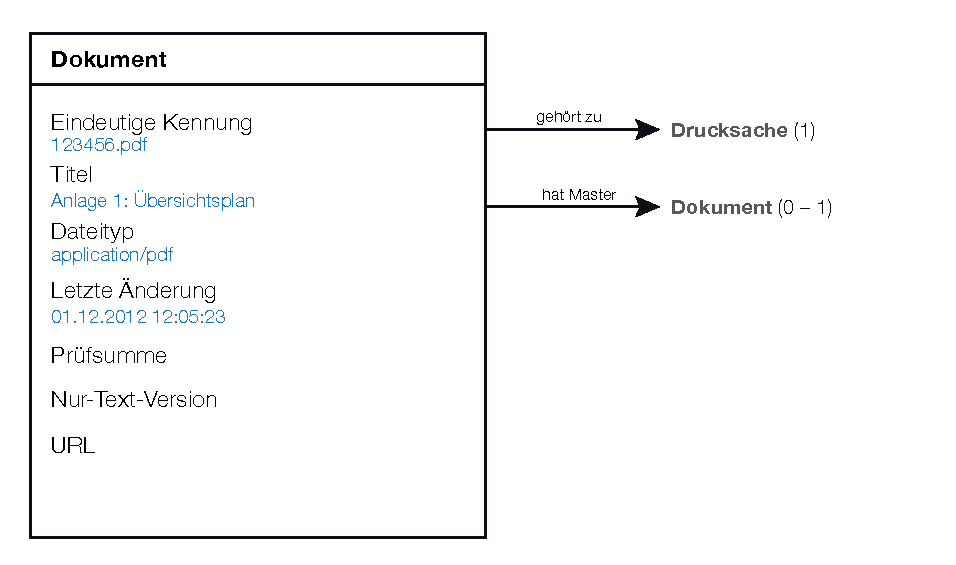
\includegraphics{images/datenmodell_dokument.pdf}
\caption{Objekttyp Dokument}
\end{figure}

\subsubsection{Eigenschaften}

\begin{description}
\item[Kennung]
Unveränderliche Kennung
\item[Titel]
Nutzerfreundliche Bezeichnung des Dokuments
\item[Dateityp]
Mime-Typ des Inhalts, z.B. ``application/x-pdf''
\item[Veröffentlichungsdatum]
Datum des Tages, an dem das Dokument ins System eingestellt wurde
\item[Änderungsdatum und -uhrzeit]
Datum und Uhrzeit der letzten Änderung des Dokuments
\item[Prüfsumme]
SHA1-Prüfsumme des Dokumenteninhalts
\item[Daten]
Der eigentliche (Binär-)Inhalt des Dokuments
\item[Nur-Text-Version]
Reine Text-Wiedergabe des Dokumenteninhalts, sofern es sich um ein
Textdokument handelt.
\end{description}

\subsubsection{Beziehungen}

\begin{itemize}
\item
  Dokumente gehören zwingend zu einer \textbf{Drucksache}, optional auch
  zu mehreren. Ein Dokument kann entweder als Hauptdokument einer
  Drucksache oder als Anlage eingestuft sein.
\item
  Ein Dokument kann auf ein anderes Dokument referenzieren, wenn es von
  dem anderen Dokument abstammt. So ist es möglich, von einem
  abgeleiteten Dokument zu seinem Dokumenten-Master zu gelangen
  (Beispiel: von einem PDF-Dokument zum OpenOffice-Original).
\end{itemize}

\subsection{Ort}

Dieser Objekttyp dient dazu, einen Ortsbezug einer Drucksache formal
abzubilden. Ortsangaben können sowohl aus Textinformationen bestehen
(beispielsweise der Name einer Straße/eines Platzes oder eine genaue
Adresse) oder aus einer Geo-Koordinatenangabe aus Längen- und
Breitengrad.

Bislang finden sich nur beim Bonner System Beispiele für Ortsangaben.

\begin{figure}[htbp]
\centering
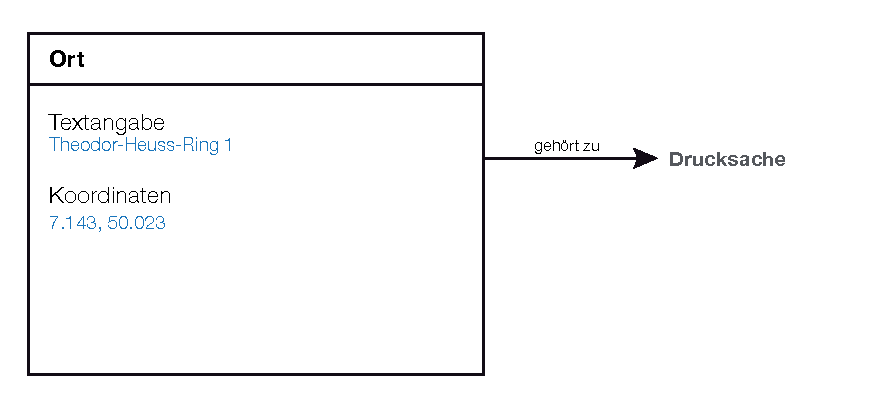
\includegraphics{images/datenmodell_ort.pdf}
\caption{Objekttyp Ort}
\end{figure}

\subsubsection{Eigenschaften}

\begin{description}
\item[Textanabe]
\emph{Optional.} Textliche Beschreibung eines Orts, z.B. in Form einer
Adresse
\item[Koordinaten]
\emph{Optional.} Längen- und Breitenangabe des Orts im WGS-84-System
{[}11{]}
\end{description}

\subsubsection{Beziehungen}

\begin{itemize}
\item
  Orte können mit Drucksachen in Verbindung stehen.
\end{itemize}

\section{Glossar}

\begin{description}
\item[AGS]
Amtlicher Gemeindeschlüssel
\item[RIS]
Ratsinformationssystem
\item[WGS 84]
World Geodetic System 1984. Ein weltweites Referenzsystem für die
Interpretation von Geokoordinaten-Angaben.
\end{description}

\section{Fußnoten}

{[}1{]}: Siehe
\href{https://www.destatis.de/DE/Methoden/Klassifikationen/Bevoelkerung/StaatsangehoerigkeitGebietsschluessel.html}{www.destatis.de/\ldots{}}

{[}2{]}: Ratsinformationssystem der Stadt Köln,
\href{http://ratsinformation.stadt-koeln.de/}{http://ratsinformation.stadt-koeln.de/}

{[}3{]}: Firma Somacos,
\href{http://www.somacos.de/de/sitzungsdienst/ratsinfo.html}{SessionNet
Produktinformation}

{[}4{]}: Ratsinformationssystem der Bezirksverwaltugn Berlin Mitte,
\href{http://www.berlin.de/ba-mitte/bvv-online/allris.net.asp}{http://www.berlin.de/\ldots{}}

{[}5{]}: CC e-gov GmbH, \href{http://www.cc-egov.de/allris.htm}{ALLRIS
Produktionformationen}

{[}6{]}: Ratsinformationssystem der Stadt Rösrath,
\href{http://212.227.97.55/ratsinfo/roesrath}{http://212.227.97.55/\ldots{}}

{[}7{]}: \href{http://www.provox.de/}{Firma PROVOX}

{[}8{]}: Ratsinformationssystem der Stadt Euskirchen,
\href{https://sitzungsdienst.euskirchen.de/}{https://sitzungsdienst.euskirchen.de/}

{[}9{]}: Firma Sternberg,
\href{http://www.sitzungsdienst.net/produkte/ratsinformationsmanagement}{SD.NET
RIM Produktionformationen}

{[}10{]}: BoRis, Ratsinformationssystem der Stadt Bonn
(Eigenentwicklung).
\href{http://www2.bonn.de/bo\_ris/ris\_sql/agm\_index.asp}{http://www2.bonn.de/\ldots{}}

{[}11{]}: World Geodetic System 1984 (EPSG:4326), wird unter anderem
auch vom Global Positioning System (GPS) verwendet.

\end{document}
